% !TeX program = xelatex
% Overleaf: Compiler = XeLaTeX; Main document = main.tex.
% Content and order follow read/analytic_continuation_brief.md only.
\RequirePackage{iftex}
\RequireXeTeX
\documentclass[aspectratio=169,11pt]{beamer}
% Portable Chinese Beamer setup: XeLaTeX + TeX Live's bundled Fandol fonts.
\usepackage[UTF8,scheme=plain,fontset=fandol]{ctex}
\usepackage{amsmath,amssymb,bm,booktabs,graphicx}
\usefonttheme{professionalfonts}
\graphicspath{{figures/}}
\definecolor{Navy}{HTML}{19334A}
\definecolor{Teal}{HTML}{078777}
\definecolor{Muted}{HTML}{607487}
\definecolor{Pale}{HTML}{EDF6F4}
\definecolor{Amber}{HTML}{B57816}
\setbeamercolor{normal text}{fg=Navy,bg=white}
\setbeamercolor{structure}{fg=Teal}
\setbeamercolor{frametitle}{fg=Navy,bg=white}
\setbeamercolor{block title}{fg=Teal,bg=Pale}
\setbeamercolor{block body}{fg=Navy,bg=Pale}
\setbeamercolor{takeaway}{fg=Navy,bg=Pale}
\setbeamercolor{alerted text}{fg=Amber}
\setbeamerfont{frametitle}{size=\large,series=\bfseries}
\setbeamerfont{block title}{size=\normalsize,series=\bfseries}
\setbeamertemplate{navigation symbols}{}
\setbeamertemplate{itemize item}{\small\textbullet}
\setbeamersize{text margin left=.75cm,text margin right=.75cm}
\setbeamertemplate{frametitle}{%
  \vspace{.08cm}\insertframetitle\par\vspace{.07cm}%
  {\color{Teal}\rule{\linewidth}{.7pt}}\vspace{-.08cm}}
\setbeamertemplate{footline}{%
  \leavevmode\hbox{%
  \begin{beamercolorbox}[wd=.87\paperwidth,ht=.30cm,dp=.15cm,leftskip=.75cm]{normal text}
    \color{Muted}\fontsize{7}{9}\selectfont
    PRB 111 保真度解析式\enspace|\enspace\insertsectionhead
  \end{beamercolorbox}%
  \begin{beamercolorbox}[wd=.13\paperwidth,ht=.30cm,dp=.15cm,rightskip=.75cm plus1fil]{normal text}
    \hfill\color{Muted}\footnotesize\insertframenumber/\inserttotalframenumber
  \end{beamercolorbox}}}
\newcommand{\takeaway}[1]{%
  \begin{beamercolorbox}[wd=\linewidth,sep=.55em]{takeaway}\small #1\end{beamercolorbox}}
\newcommand{\source}[1]{{\par\vspace{.08cm}\fontsize{7.5}{10}\selectfont\color{Muted}#1\par}}
\newcommand{\ket}[1]{\lvert #1\rangle}
\newcommand{\bra}[1]{\langle #1\rvert}
\newcommand{\iu}{\mathrm{i}}
\newcommand{\Q}{\mathcal Q}
\newcommand{\ff}{\mathfrak f}
\DeclareMathOperator{\tr}{tr}
\hypersetup{colorlinks=true,urlcolor=Teal,
  pdftitle={非理想 Majorana 编织的保真度解析式},
  pdfsubject={PRB 111 模型：低能投影、解析延拓、验证与误差}}

\newcommand{\PresenterName}{}
\newcommand{\PresentationDate}{}

\begin{document}

% 01 — Cover
\begin{frame}[plain]
  \vspace{.65cm}
  {\color{Teal}\large 解析式结果汇报}\par\vspace{.45cm}
  {\huge\bfseries 非理想 Majorana 编织\\[.2cm]保真度的解析公式}\par
  \vspace{.35cm}
  {\large PRB 111 模型：低能投影与解析延拓}\par
  \vspace{.4cm}{\color{Teal}\rule{2.5cm}{2pt}}\par\vspace{.3cm}
  \PresenterName\quad\PresentationDate\par\vspace{.4cm}
  \small
  问题与模型\quad$\longrightarrow$\quad 完整结果公式\quad$\longrightarrow$\quad 推导主线\par\medskip
  结果分析\quad$\longrightarrow$\quad 图像与验证\quad$\longrightarrow$\quad 近似条件
\end{frame}

\section{1. 问题与模型}

% 02 — brief §1: question, comparison and overall idea
\begin{frame}[t]{1. 问题与模型：研究问题与思路}
  \textbf{当 $E_1$ 和 $t_1$ 同时非零时，能否写出具体保真度公式，并解释 Fig. 1(d)？}
  \vspace{.15cm}
  \begin{center}
    \small\renewcommand{\arraystretch}{1.35}
    \begin{tabular}{p{2.0cm}p{4.6cm}p{5.6cm}}
      \toprule & 2008.pdf 的几何思路 & 当前推导\\\midrule
      找计算空间 & 随参数变化的简并基态空间 & 强耦合确定低能空间，再投影弱耦合\\
      描述几何 & Berry 联络、曲率 & 连续平行输运基底及闭环变化\\
      得到几何门 & holonomy & 终点相对起点的基底旋转 $B$\\
      内部动力学 & 理想方案只有共同相位 & 非零 $E_1,t_1$ 的动态作用必须保留\\\bottomrule
    \end{tabular}
  \end{center}
  \small
  \textbf{推导路线：}分清辅助与剩余模式，保持辅助模式低能占据；在移动基底中求解三段传播，其中第二段用参数延拓；最后换回起点基底并执行两圈。
  \vspace{.15cm}
  解析式保留低能模型内的全部累计相位；完整模型修正另行估价。
  \source{2008.pdf：Holonomic implementation of CNOT gate on topological Majorana qubits，SciPost Phys. Core 3, 014 (2020)。}
\end{frame}

% 03 — brief §1: model and readout
\begin{frame}[t]{1. 问题与模型：哈密顿量与读出}
  取 $\{\gamma_i,\gamma_j\}=2\delta_{ij}$，模型为
  \[
    H=\iu\gamma_a(d\gamma_b+u_2\gamma_2-u_3\gamma_3)
      +\iu\gamma_1(u_1\gamma_b+e\gamma_2).
  \]
  \[
    d=E_d,\qquad e=E_1,\qquad \eta=|t_1|_{\max},\qquad
    u_j(t)=|t_j(t)|,\qquad E_0=t_c=C.
  \]
  每段持续 $\tau$，三段完成一次交换；连续两圈共 $6\tau$。
  \vspace{.2cm}
  \begin{block}{沿用原文指定初末态的读出}
    \[
      f_{\rm full}=|\langle\psi_1^+(0)|\psi_1^-(6\tau)\rangle|.
    \]
    $f_0$ 表示低能解析公式，完整模型与其差别记为
    \[
      f_{\rm full}=f_0+\Delta_{\rm phys}.
    \]
  \end{block}
  \source{模型来源：Phys. Rev. B 111, 205411 (2025)。本报告研究该三段协议下的指定读出。}
\end{frame}

% 04 — brief §1: pulse table
\begin{frame}[t]{1. 问题与模型：三段控制协议}
  每段局部时间 $s\in[0,1]$，定义
  \[
    a(s)=\frac{1-\cos\pi s}{2},\qquad b=1-a,\qquad
    q=\sqrt{a^2+b^2},\qquad g=\frac aq.
  \]
  \begin{center}
    \renewcommand{\arraystretch}{1.5}
    \begin{tabular}{ccccc}
      \toprule 控制段 & $d$ & $u_2$ & $u_3$ & $u_1$\\\midrule
      I & $Cb$ & $Ca$ & $0$ & $\eta a$\\
      II & $0$ & $Cb$ & $Ca$ & $\eta b$\\
      III & $Ca$ & $0$ & $Cb$ & $0$\\\bottomrule
    \end{tabular}
  \end{center}
  \vspace{.25cm}
  \takeaway{以下结果使用这套原三段门控；$u_1$ 与 $u_2$ 联动。弱耦合改变低能内部动力学，强控制决定参考低能空间。}
\end{frame}

% 05 — brief §1: feasibility of the parallel-transport frame, before the result
\begin{frame}[t]{1. 为什么可以选择平行输运标架？}
  \small
  \setlength{\abovedisplayskip}{4pt}\setlength{\belowdisplayskip}{4pt}
  \textbf{投影确定低能空间；我们再选择基底随空间移动，同时不在空间内部额外转动。}
  当前强耦合参考模型的辅助能隙不闭合：
  \[
    R=\sqrt{d^2+u_2^2+u_3^2}=Cq\ge C/\sqrt2>0.
  \]
  因此参考投影光滑、维数不变；给定起点基底后，可沿路径连续构造
  \[
    \Q=(\ket{q_0},\ket{q_1}),\qquad
    \boxed{\langle q_i|\dot q_j\rangle=0\ \Longleftrightarrow\ \Q^\dagger\dot\Q=0.}
  \]
  条件只要求基底的变化在当前低能空间内部没有分量；基底本身仍随空间移动。
  闭环后，局部平行允许留下净几何变换：
  \[
    \Q(T)=\Q(0)B.
  \]
  下一页直接检验原三段协议的模式标架，包含第二、第三段及段间衔接。
  \vspace{.15cm}
  \takeaway{平行是基底的选择，不增加物理近似。弱耦合与辅助绝热条件控制低能约化的准确性；实际态仍受 $h_K$ 驱动。}
\end{frame}

% 06 — brief §1: explicit checks for all three segments and both joins
\begin{frame}[t]{1. 三段标架的平行性与连续性}
  \small
  \setlength{\abovedisplayskip}{4pt}\setlength{\belowdisplayskip}{4pt}
  每段令 $c_\theta=\cos\theta=b/q$、$s_\theta=\sin\theta=a/q$，局部角从 $0$ 到 $\pi/2$。
  向量均写在固定坐标 $(\gamma_b,\gamma_2,\gamma_3)$ 中，点号表示物理时间导数：
  \begin{center}
    \scriptsize\renewcommand{\arraystretch}{1.4}
    \setlength{\tabcolsep}{5pt}
    \begin{tabular}{cccccc}
      \toprule 段 & $\bm n$ & $\bm f_1$ & $\bm f_2$ & $\dot{\bm f}_1$ & $\dot{\bm f}_2$\\\midrule
      I & $(c_\theta,s_\theta,0)$ & $(-s_\theta,c_\theta,0)$ & $(0,0,1)$ & $-\dot\theta\bm n$ & $0$\\
      II & $(0,c_\theta,-s_\theta)$ & $(-1,0,0)$ & $(0,s_\theta,c_\theta)$ & $0$ & $\dot\theta\bm n$\\
      III & $(s_\theta,0,-c_\theta)$ & $(-c_\theta,0,-s_\theta)$ & $(0,1,0)$ & $\dot\theta\bm n$ & $0$\\\bottomrule
    \end{tabular}
  \end{center}
  导数均为零或沿法向，而 $\bm f_i\cdot\bm n=0$，故每段均满足
  \[
    \boxed{\bm f_i\cdot\dot{\bm f}_j=0,\qquad i,j=1,2.}
  \]
  前段终点 $\theta=\pi/2$ 与后段起点 $\theta=0$ 给出相同标架：
  \begin{center}
    \scriptsize\renewcommand{\arraystretch}{1.3}
    \begin{tabular}{cccc}
      \toprule 接点 & 共同的 $\bm n$ & 共同的 $\bm f_1$ & 共同的 $\bm f_2$\\\midrule
      I 终点 = II 起点 & $(0,1,0)$ & $(-1,0,0)$ & $(0,0,1)$\\
      II 终点 = III 起点 & $(0,0,-1)$ & $(-1,0,0)$ & $(0,1,0)$\\\bottomrule
    \end{tabular}
  \end{center}
  \takeaway{三段逐段平行且连续；局部角从零开始不重置标架。相应多体基底取连续的平行输运约定，满足 $\Q^\dagger\dot\Q=0$。}
\end{frame}

\section{2. 完整结果公式}

% 07 — brief §2: the complete result, before derivation
\begin{frame}[t]{2. 完整结果公式：先给出最终读出}
  \small
  \[
    \alpha=\frac{E_1\tau}{\hbar},\qquad \nu=\frac{\eta\tau}{\hbar},\qquad
    j=\int_0^1\frac{a^2}{q}\,ds=\frac{\mathsf E(1/2)}\pi,\qquad
    k=\int_0^1\frac bq\,ds=\frac{\mathsf K(1/2)}\pi.
  \]
  $\mathsf E,\mathsf K$ 为参数 $m=1/2$ 的完全椭圆积分；
  $j\simeq0.4299233$、$k\simeq0.5901703$。
  \vspace{.15cm}
  \[
    \boxed{f_0=\ff(\alpha,\nu)
       =4(1-|\beta|^2)\left[\operatorname{Im}(e^{-\iu\delta}\beta)\right]^2.}
  \]
  \[
  \begin{aligned}
    \beta&=-\frac{e^{-\iu\nu/2}\mathsf S_\nu(\alpha;1)
                  +\iu e^{\iu\nu/2}\mathsf C_\nu(\alpha;1)^*}{\sqrt2},\\[.15cm]
    \delta&=(1+k)\alpha-j\nu.
  \end{aligned}
  \]
  \vspace{.15cm}
  \takeaway{$\mathsf C,\mathsf S$ 的定义见下一页。若使用重叠模的平方，则 $F_0=f_0^2$；后面的图比较 $f$。}
\end{frame}

% 08 — brief §2: definitions and convergence
\begin{frame}[t]{2. 完整结果公式：特殊函数的定义}
  \small
  \setlength{\abovedisplayskip}{5pt}\setlength{\belowdisplayskip}{5pt}
  \setlength{\abovedisplayshortskip}{3pt}\setlength{\belowdisplayshortskip}{3pt}
  \[
    P(s)=\int_0^s b(u)\,du=\frac s2+\frac{\sin\pi s}{2\pi},\qquad J_0=1.
  \]
  \[
  \begin{aligned}
    J_m(s;\nu)={}&\int_{0<s_m<\cdots<s_1<s}
       \left[\prod_{\ell=1}^m g(s_\ell)\right]\\[-.1cm]
       &\times\exp\!\left[2\iu\nu\sum_{\ell=1}^m(-1)^{\ell+1}P(s_\ell)\right]
          \,ds_1\cdots ds_m.
  \end{aligned}
  \]
  \[
  \begin{aligned}
    \mathsf C_\nu(\alpha;s)&=\sum_{n=0}^\infty(-1)^n\alpha^{2n}J_{2n}(s;\nu),\\
    \mathsf S_\nu(\alpha;s)&=\sum_{n=0}^\infty(-1)^n\alpha^{2n+1}J_{2n+1}(s;\nu).
  \end{aligned}
  \]
  \[
    |J_m(s;\nu)|\le\frac{G(s)^m}{m!},\qquad G(s)=\int_0^s g(u)\,du
    \quad(\nu\text{ 为实数}).
  \]
  \textbf{核全部已知，级数对任意有限累计角收敛。}
  $J_m$ 表示在已包含 $t_1$ 演化的背景下，$E_1$ 产生的第 $m$ 阶相干作用。
\end{frame}

\section{3. 推导主线}

% 09 — brief §3, step 1
\begin{frame}[t]{3.1 拆分强、弱耦合：确定辅助模式}
  \[
    H=H_0+V,\qquad
    H_0=\iu\gamma_a(d\gamma_b+u_2\gamma_2-u_3\gamma_3),\qquad
    V=\iu\gamma_1(u_1\gamma_b+e\gamma_2).
  \]
  换元后，强耦合部分写为
  \[
    H_0=\iu R\gamma_a\gamma_c,\qquad
    R=\sqrt{d^2+u_2^2+u_3^2},\qquad
    \gamma_c=\frac{d\gamma_b+u_2\gamma_2-u_3\gamma_3}{R}.
  \]
  \begin{itemize}\setlength{\itemsep}{.2cm}
    \item $\gamma_a,\gamma_c$ 形成辅助模式，激发能为 $2R$。
    \item 当前路径上 $R\ge C/\sqrt2$，强耦合能隙始终存在。
    \item 弱耦合远小于 $C$、控制相对辅助能隙足够慢时，近似保持辅助模式低能占据。
  \end{itemize}
  \vspace{.2cm}
  \takeaway{拆分和换元本身是精确的；近似发生在忽略辅助模式的激发及相关修正时。}
\end{frame}

% 10 — brief §3, step 1: weak projection
\begin{frame}[t]{3.1 低能投影：保留弱耦合的内部作用}
  \small
  \setlength{\abovedisplayskip}{5pt}\setlength{\belowdisplayskip}{5pt}
  令 $\bm\Gamma=(\gamma_b,\gamma_2,\gamma_3)$、$\bm n=(d,u_2,-u_3)/R$。
  在垂直于 $\bm n$ 的平面内选连续平行输运方向 $\bm f_1,\bm f_2$，定义
  \[
    \widetilde\gamma_2=\bm f_1\cdot\bm\Gamma,\qquad
    \widetilde\gamma_3=\bm f_2\cdot\bm\Gamma,\qquad
    \bm w=(u_1,e,0),\quad \omega=\bm w\cdot\bm n,\quad w_i=\bm w\cdot\bm f_i.
  \]
  \[
    V=\underbrace{\iu\omega\gamma_1\gamma_c}_{V_{\rm off}}
       +\underbrace{\iu\gamma_1(w_1\widetilde\gamma_2+w_2\widetilde\gamma_3)}_{V_{\rm in}}.
  \]
  \[
    P_0=\frac{1-\iu\gamma_a\gamma_c}{2},\qquad
    P_0V_{\rm off}P_0=0,\qquad P_0VP_0=P_0V_{\rm in}P_0.
  \]
  在随动逻辑基底中，$-\iu\gamma_1\widetilde\gamma_2\leftrightarrow Z$、
  $-\iu\widetilde\gamma_3\gamma_1\leftrightarrow Y$。去掉共同能量后，
  \[
    \boxed{h_K=-w_1Z+w_2Y.}
  \]
  直接投影为零是代数关系；忽略 $V_{\rm off}$ 的间接修正与激发是近似。
  $Z$ 产生相对相位，$Y$ 混合逻辑态。
\end{frame}

% 11 — brief §3, step 1: geometry figure
\begin{frame}[t]{3.1 平行输运标架的几何图}
  \begin{center}
    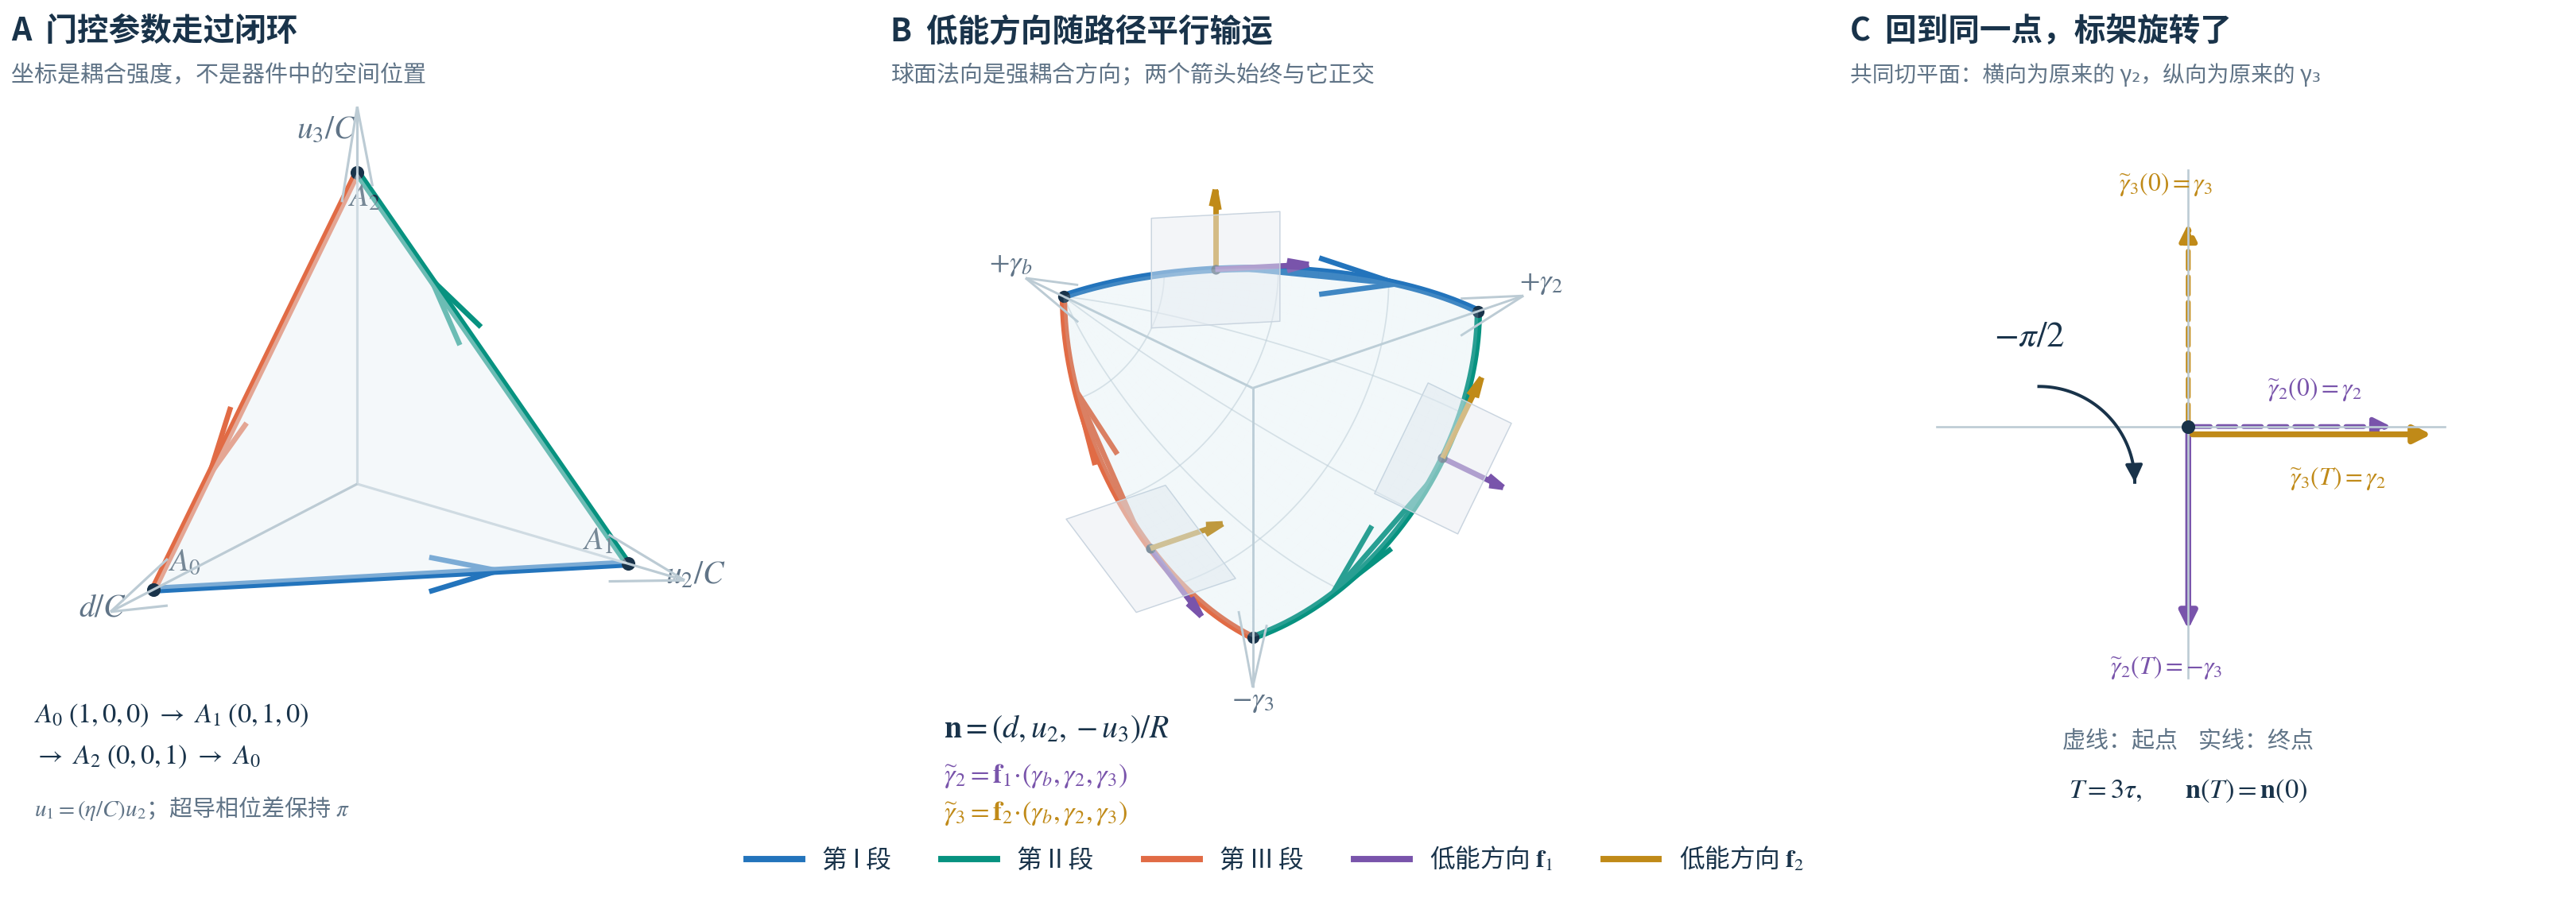
\includegraphics[width=\linewidth,height=4.25cm,keepaspectratio]{frame_panels.png}
  \end{center}
  \small
  \textbf{左：}强控制参数路径。\quad
  \textbf{中：}$\bm n=(d,u_2,-u_3)/R$ 及两个正交的低能模式方向。\par\medskip
  \textbf{右：}控制闭合后，平行输运标架净转过 $-\pi/2$，产生 holonomy。
  \vspace{.12cm}
  \takeaway{两根箭头用于构造逻辑基底 $\Q(t)$，不直接代表两列多体态；几何图描述强耦合参考空间。}
\end{frame}

% 12 — brief §3, step 2: effective Hamiltonians
\begin{frame}[t]{3.2 求解三段动态传播}
  将原脉冲和连续标架代入，三段有效 Hamiltonian 为
  \[
    \boxed{
    h_{\rm I}=\frac{\eta a^2-eb}{q}Z,\qquad
    h_{\rm II}=\eta bZ+egY,\qquad h_{\rm III}=eY.}
  \]
  第一、三段各自只有一个固定逻辑轴，可直接积分：
  \[
    D_1=e^{-\iu(j\nu-k\alpha)Z},\qquad D_3=e^{-\iu\alpha Y}.
  \]
  第二段的 $Z,Y$ 系数比例随时间改变，不同时刻的 Hamiltonian 一般不对易：
  \[
    \iu\partial_s D_2(s)=[\nu b(s)Z+\alpha g(s)Y]D_2(s),\qquad D_2(0)=I.
  \]
  \small 这里 $s$ 是段内无量纲时间，$\partial_s$ 是时间导数；$D_1,D_3$ 表示各段终点传播。
  \vspace{.15cm}
  \takeaway{先得到低能有效模型，再构造其第二段传播。以下参数延拓不改变这一步物理近似。}
\end{frame}

% 13 — brief §3, step 2: continuation
\begin{frame}[t]{3.2 从 $E_1=0$ 延拓到目标参数}
  \small
  \setlength{\abovedisplayskip}{5pt}\setlength{\belowdisplayskip}{5pt}
  固定 $\eta,\tau$ 和波形，取 $E(x)=xE_1$；$s$ 为时间，$x$ 为参数：
  \[
    \iu\partial_sD_2(s;x)=[\nu b(s)Z+x\alpha g(s)Y]D_2(s;x),\qquad D_2(0;x)=I.
  \]
  \[
    D_{\rm ref}(s)=D_2(s;0)=e^{-\iu\nu P(s)Z},\qquad
    D_2(s;x)=D_{\rm ref}(s)W(s;x).
  \]
  \[
    \partial_sW=x\alpha M(s)W,\quad W(0;x)=I,\qquad
    M(s)=\begin{pmatrix}0&-g e^{2\iu\nu P}\\g e^{-2\iu\nu P}&0\end{pmatrix}.
  \]
  按 $x$ 展开，各阶系数由对时间 $s$ 的积分确定：
  \[
    \begin{aligned}
      W(s;x)&=\sum_{m=0}^{\infty}x^m W_m(s),\qquad W_0=I,\\
      W_m(s)&=\alpha\int_0^s M(u)W_{m-1}(u)\,du\qquad(m\ge1).
    \end{aligned}
  \]
  取 $x=1$ 并按奇偶阶整理，即得到第 2 部分的 $\mathsf C,\mathsf S$。
  \source{$D_1,D_3$ 也要同步替换 $\alpha\to x\alpha$。这是全阶 Taylor/Dyson 构造；模型方程决定全部系数，仅凭 $x=0$ 的解值不足以确定结果。}
\end{frame}

% 14 — brief §3, step 3: why two states
\begin{frame}[t]{3.3 组合动态传播：为什么只有两个低能态？}
  \small
  \setlength{\abovedisplayskip}{5pt}\setlength{\belowdisplayskip}{5pt}
  六个 Majorana（含旁观 $\gamma_4$）两两配对，得到三个费米子模式：
  \[
    f_{\rm aux}=\frac{\gamma_a+\iu\gamma_c}{2},\qquad
    f_L=\frac{\gamma_1+\iu\widetilde\gamma_2}{2},\qquad
    f_R=\frac{\widetilde\gamma_3+\iu\gamma_4}{2}.
  \]
  总宇称守恒，以固定偶宇称为例；能量只由辅助占据决定：
  \[
    (-1)^{n_{\rm aux}+n_L+n_R}=+1,\qquad H_0=R(2n_{\rm aux}-1).
  \]
  {\centering
    \renewcommand{\arraystretch}{1.15}
    \begin{tabular}{cccc}
      \toprule 偶宇称态 $\ket{n_{\rm aux},n_L,n_R}$ & 辅助占据 & $H_0$ 能量 & 低能投影\\\midrule
      $\ket{0,0,0}$ & $0$ & $-R$ & 保留为 $\ket{0_L}$\\
      $\ket{0,1,1}$ & $0$ & $-R$ & 保留为 $\ket{1_L}$\\
      $\ket{1,0,1}$ & $1$ & $+R$ & 排除\\
      $\ket{1,1,0}$ & $1$ & $+R$ & 排除\\\bottomrule
    \end{tabular}\par}
  \vspace{.1cm}
  \textbf{固定宇称后的四态中，两态辅助未激发；另外两态高出 $2R$。}
  $H_0$ 不依赖 $n_L,n_R$，所以 $\ket{0,1,1}$ 与 $\ket{0,0,0}$ 同样低能。
  \source{奇宇称扇区也保留两个态；若不固定总宇称，辅助未激发的空间是四维。加入 $V$ 可劈裂保留的两态，不要求完整 $H$ 保持二重简并。}
\end{frame}

% 15 — brief §3, step 3: Q and the explicit removal of the common phase
\begin{frame}[t]{3.3 移动基底与共同相位的提取}
  \small
  \setlength{\abovedisplayskip}{4pt}\setlength{\belowdisplayskip}{4pt}
  上页二维空间取平行输运基底，$\Q$ 为 $4\times2$ 矩阵。原始系数记为 $c_{\rm raw}$：
  \[
    \Q(t)=\begin{pmatrix}\ket{q_0(t)}&\ket{q_1(t)}\end{pmatrix},\qquad
    \ket{\psi(t)}\simeq\Q(t)c_{\rm raw}(t).
  \]
  $\Q^\dagger\Q=I_2$，$\Q\Q^\dagger=P_0$，$\Q^\dagger\dot\Q=0$；两列均满足
  $H_0\ket{q_j}=-R\ket{q_j}$。代入薛定谔方程并投影：
  \[
    \iu\hbar\dot c_{\rm raw}=(-RI_2+h_K)c_{\rm raw},\qquad h_K=\Q^\dagger V\Q.
  \]
  显式提取共同能量 $-R(t)$ 产生的整体相位：
  \[
    c_{\rm raw}(t)=e^{\iu\Phi(t)}c(t),\qquad
    \Phi(t)=\frac1\hbar\int_0^tR(u)\,du,\qquad c_{\rm raw}(0)=c(0).
  \]
  两边代入后，$-Rc$ 抵消：
  \[
    e^{\iu\Phi}(-Rc+\iu\hbar\dot c)=e^{\iu\Phi}(-Rc+h_Kc)
    \quad\Longrightarrow\quad \boxed{\iu\hbar\dot c=h_Kc.}
  \]
  \source{后续 $D_j$ 求解的是 $c$。提取共同相位在投影模型内严格成立；$h_K$ 中的相对相位与态混合仍全部保留。}
\end{frame}

% 16 — brief §3, step 3: BD product with the common phase restored
\begin{frame}[t]{3.3 换回起点基底：得到 $BD_3D_2D_1$}
  \small
  \setlength{\abovedisplayskip}{5pt}\setlength{\belowdisplayskip}{5pt}
  提取共同相位后的系数，以及终点的基底，分别满足
  \[
    c(T)=D_3D_2D_1c(0),\qquad
    \Q(T)=\Q(0)B,\qquad B=e^{\iu\pi X/4},\quad T=3\tau.
  \]
  这里 $X=-\iu\gamma_2\gamma_3$。把共同相位一起代入物理终态：
  \[
  \begin{aligned}
    \ket{\psi(T)}&\simeq\Q(T)c_{\rm raw}(T)\\
                &=e^{\iu\Phi(T)}\Q(T)D_3D_2D_1c(0)\\
                &=e^{\iu\Phi(T)}\Q(0)BD_3D_2D_1c(0).
  \end{aligned}
  \]
  \[
    U_{\rm low}(T)=e^{\iu\Phi(T)}U_{\rm cyc},\qquad
    \boxed{U_{\rm cyc}=BD_3D_2D_1,\quad U_{\rm two}=U_{\rm cyc}^2.}
  \]
  任意低能初态 $\ket{i}$ 与目标态 $\ket{f}$ 的跃迁模满足
  \[
    |\bra{f}U_{\rm low}\ket{i}|=|e^{\iu\Phi(T)}\bra{f}U_{\rm cyc}\ket{i}|
    =|\bra{f}U_{\rm cyc}\ket{i}|.
  \]
  \takeaway{这里只做代入，没有交换矩阵，因此不要求 $H_0,V$ 对易。$B$ 换坐标，$D_j$ 求内部动态；一般不能把两圈写成 $B^2(D_3D_2D_1)^2$。}
\end{frame}

% 17 — brief §3, step 3: readout
\begin{frame}[t]{3.3 用哈密顿--凯莱恒等式得到保真度}
  \small
  \setlength{\abovedisplayskip}{5pt}\setlength{\belowdisplayskip}{5pt}
  记 $U=U_{\rm cyc}=BD_3D_2D_1$。去掉共同相位后，$U\in SU(2)$。
  直接相乘，用第 2 部分已定义的 $\beta,\delta$ 整理：
  \[
    U_{11}=-\iu e^{\iu\delta}\beta^*,\qquad U_{22}=U_{11}^*,\qquad
    |U_{12}|^2=1-|\beta|^2.
  \]
  \[
    \tr U=U_{11}+U_{22}=-2\operatorname{Im}(e^{-\iu\delta}\beta).
  \]
  二阶矩阵的哈密顿--凯莱恒等式，结合 $\det U=1$，给出
  \[
    U^2-(\tr U)U+I=0
    \quad\Longrightarrow\quad (U^2)_{12}=(\tr U)U_{12}.
  \]
  因 $U_{\rm two}=U^2$，在当前投影与读出约定下，
  \[
    \boxed{\begin{aligned}
      f_0=|(U^2)_{12}|^2
         &=|\tr U|^2\,|U_{12}|^2\\
         &=4(1-|\beta|^2)[\operatorname{Im}(e^{-\iu\delta}\beta)]^2.
    \end{aligned}}
  \]
\end{frame}

\section{4. 结果分析}

% 18 — brief §4.1: first limit
\begin{frame}[t]{4.1 极限一：$E_1=t_1=0$}
  固定强控制 $C$、段时长 $\tau$ 和三段路径，令 $\alpha=\nu=0$。
  \[
    \mathsf C_0(0;1)=1,\qquad\mathsf S_0(0;1)=0,\qquad
    \beta=-\frac{\iu}{\sqrt2},\qquad\delta=0.
  \]
  代回主公式：
  \[
    \boxed{f_0(0,0)=4\left(1-\frac12\right)\frac12=1,\qquad F_0(0,0)=1.}
  \]
  从传播矩阵看，
  \[
    D_1=D_2=D_3=I,\qquad U_{\rm cyc}=B,\qquad U_{\rm two}=B^2=\iu X.
  \]
  \vspace{.25cm}
  \takeaway{恢复理想编织，将指定初态翻转到目标态。这里 $t_1=0$ 指额外门控为零，编织所需的强控制仍照常变化。}
\end{frame}

% 19 — brief §4.1: second limit
\begin{frame}[t]{4.1 极限二：仅 $E_1=0$}
  \small
  此时 $\alpha=0$，$\nu=\eta\tau/\hbar$ 可为任意有限值。定义
  \[
    \Theta=(\tfrac12+j)\nu,\qquad
    \beta=-\frac{\iu}{\sqrt2}e^{\iu\nu/2},\qquad\delta=-j\nu.
  \]
  有效 Hamiltonian 也直接给出
  \[
    D_1=e^{-\iu j\nu Z},\quad D_2=e^{-\iu\nu Z/2},\quad D_3=I,
    \qquad U_{\rm cyc}=Be^{-\iu\Theta Z}.
  \]
  \[
    \boxed{f_0(0,\nu)=\cos^2\Theta,\qquad F_0(0,\nu)=\cos^4\Theta.}
  \]
  \[
    f_0=1-\Theta^2+\frac{\Theta^4}{3}+O(\Theta^6),\qquad
    F_0=1-2\Theta^2+\frac{5\Theta^4}{3}+O(\Theta^6).
  \]
  \textbf{完整余弦不是小角近似；其展开与独立微扰结果一致。}
  $\Theta=n\pi$ 时恢复 $f_0=1$，半整数倍 $\pi$ 时为零。
  \source{两种极限都在低能有效模型内成立，完整五模仍可能有有限速度偏差。另一参数轴 $\eta=0$ 有 $f_0=\cos^2[(1+2k)\alpha]$。}
\end{frame}

% 20 — brief §4.2
\begin{frame}[t]{4.2 峰位与峰高来自两个不同因素}
  令 $p=|\beta|^2$、$\chi=\arg\beta-\delta$，同一结果可写为
  \[
    \boxed{f_0=\underbrace{4p(1-p)}_{\mathcal V}\sin^2\chi.}
  \]
  \begin{itemize}\setlength{\itemsep}{.2cm}
    \item $\chi$ 描述振荡相位，$\mathcal V$ 限制峰高；两者都随参数变化。
    \item $Y,Z$ 不对易，使复系数 $\beta$ 的模和相位一起变化，曲线一般不再是等幅余弦。
    \item 固定正有限比例 $r=\eta/E_1$ 时，低能模型长时给出 $f_0=O_r(\alpha^{-4})$。
  \end{itemize}
  \vspace{.15cm}
  \takeaway{衰减可以来自相干演化，无需引入耗散；它不直接保证有限 $C$ 完整模型的无限时行为。}
  \source{$\beta=0$ 时直接使用主公式，不取无定义的相位。实际峰位还受随参数变化的包络影响。}
\end{frame}

% 21 — brief §4.3
\begin{frame}[t]{4.3 中间高保真度区域：二阶抵消}
  \small
  令 $\mathcal A=\tfrac12+j$、$\mathcal B=1+2k$，小累计角下
  \[
    f_0=1-(\mathcal B\alpha-\mathcal A\nu)^2
          +O\!\left((|\alpha|+|\nu|)^4\right).
  \]
  当
  \[
    \boxed{r=r_*\equiv\frac{\eta}{E_1}
      =\frac{1+2k}{1/2+j}\simeq2.3446,}
  \]
  二阶损失消失，但仍有四阶残余：
  \[
    1-f_0=4J_p^2\alpha^2\nu^2+O\!\left((|\alpha|+|\nu|)^6\right),\qquad
    J_p=2\int_0^1g(s)\!\int_s^1b(u)\,du\,ds>0.
  \]
  \vspace{.15cm}
  \takeaway{这是一条指定读出的二阶抵消线，使初始区域更平坦；不意味着全时间保真度为一，也不意味着整个逻辑门无误差。}
  \source{一般双参数展开的全部四阶系数，已与独立微扰结果逐项核对。}
\end{frame}

\section{5. 图像与验证结果}

% 22 — brief §5: first image
\begin{frame}[t]{5. 图像与验证：论文与解析公式热图}
  \begin{center}
    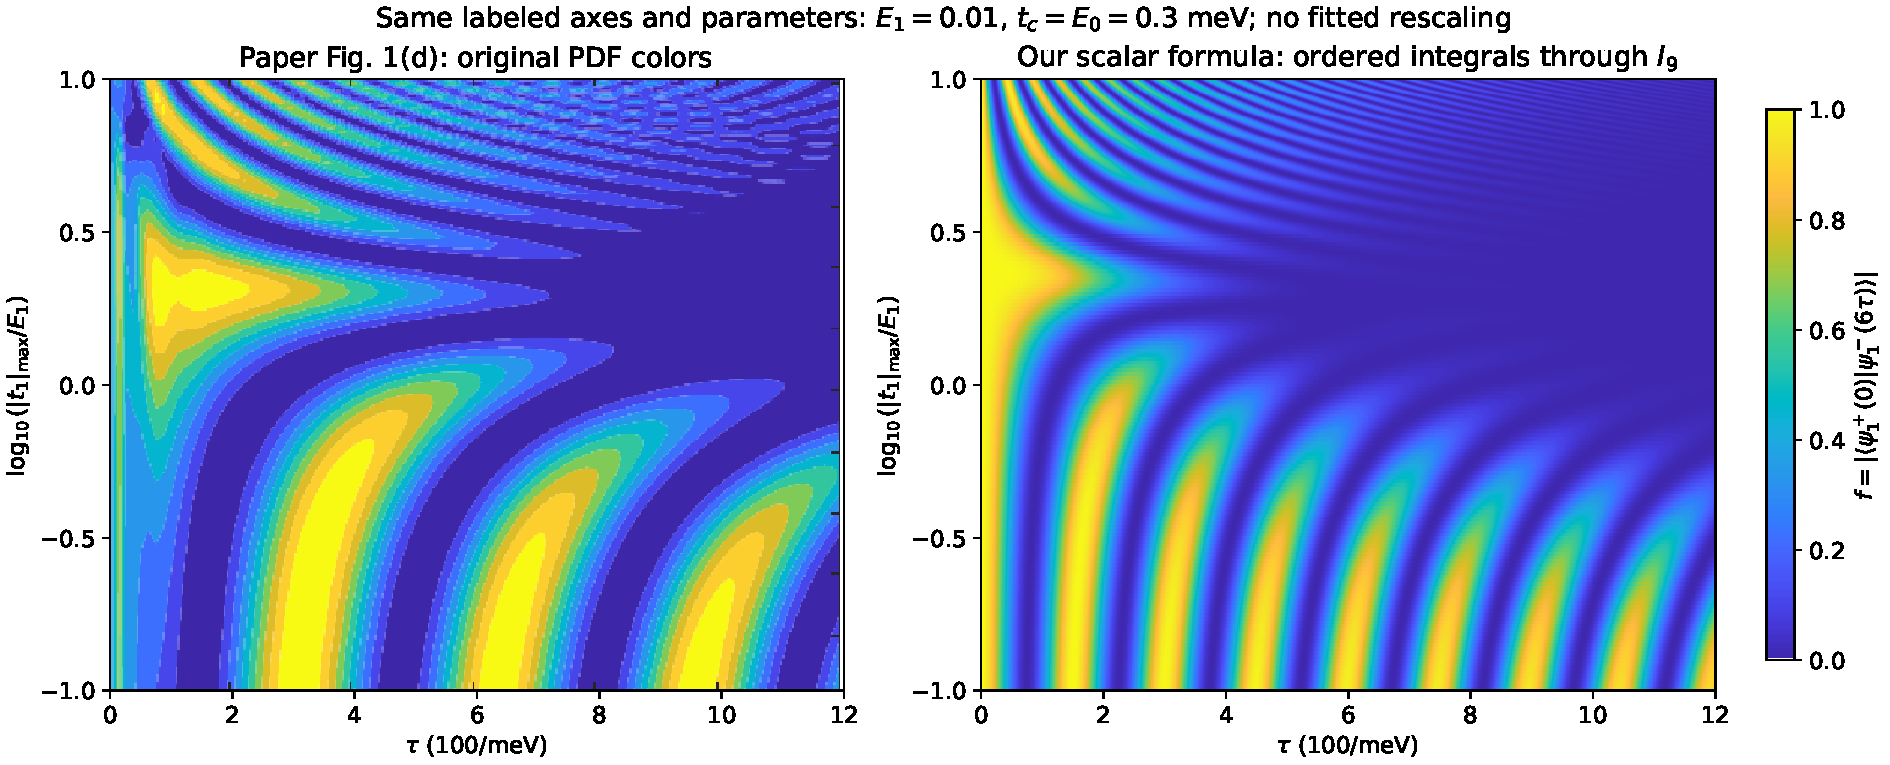
\includegraphics[width=\linewidth,height=4.65cm,keepaspectratio]{paper_vs_formula.pdf}
  \end{center}
  \small
  $E_1=0.01\,\mathrm{meV}$、$C=0.3\,\mathrm{meV}$；横轴 $\lambda=E_1\tau/\hbar$，纵轴 $\log_{10}r$。
  \vspace{.12cm}
  \takeaway{公式解释单参数主导区的振荡、中间区域的变化，以及峰位、峰高的共同演化。与论文图比较的是趋势。}
\end{frame}

% 23 — brief §5: factor-2 image stays here
\begin{frame}[t]{5. 图像与验证：因子 2 的试画}
  \begin{center}
    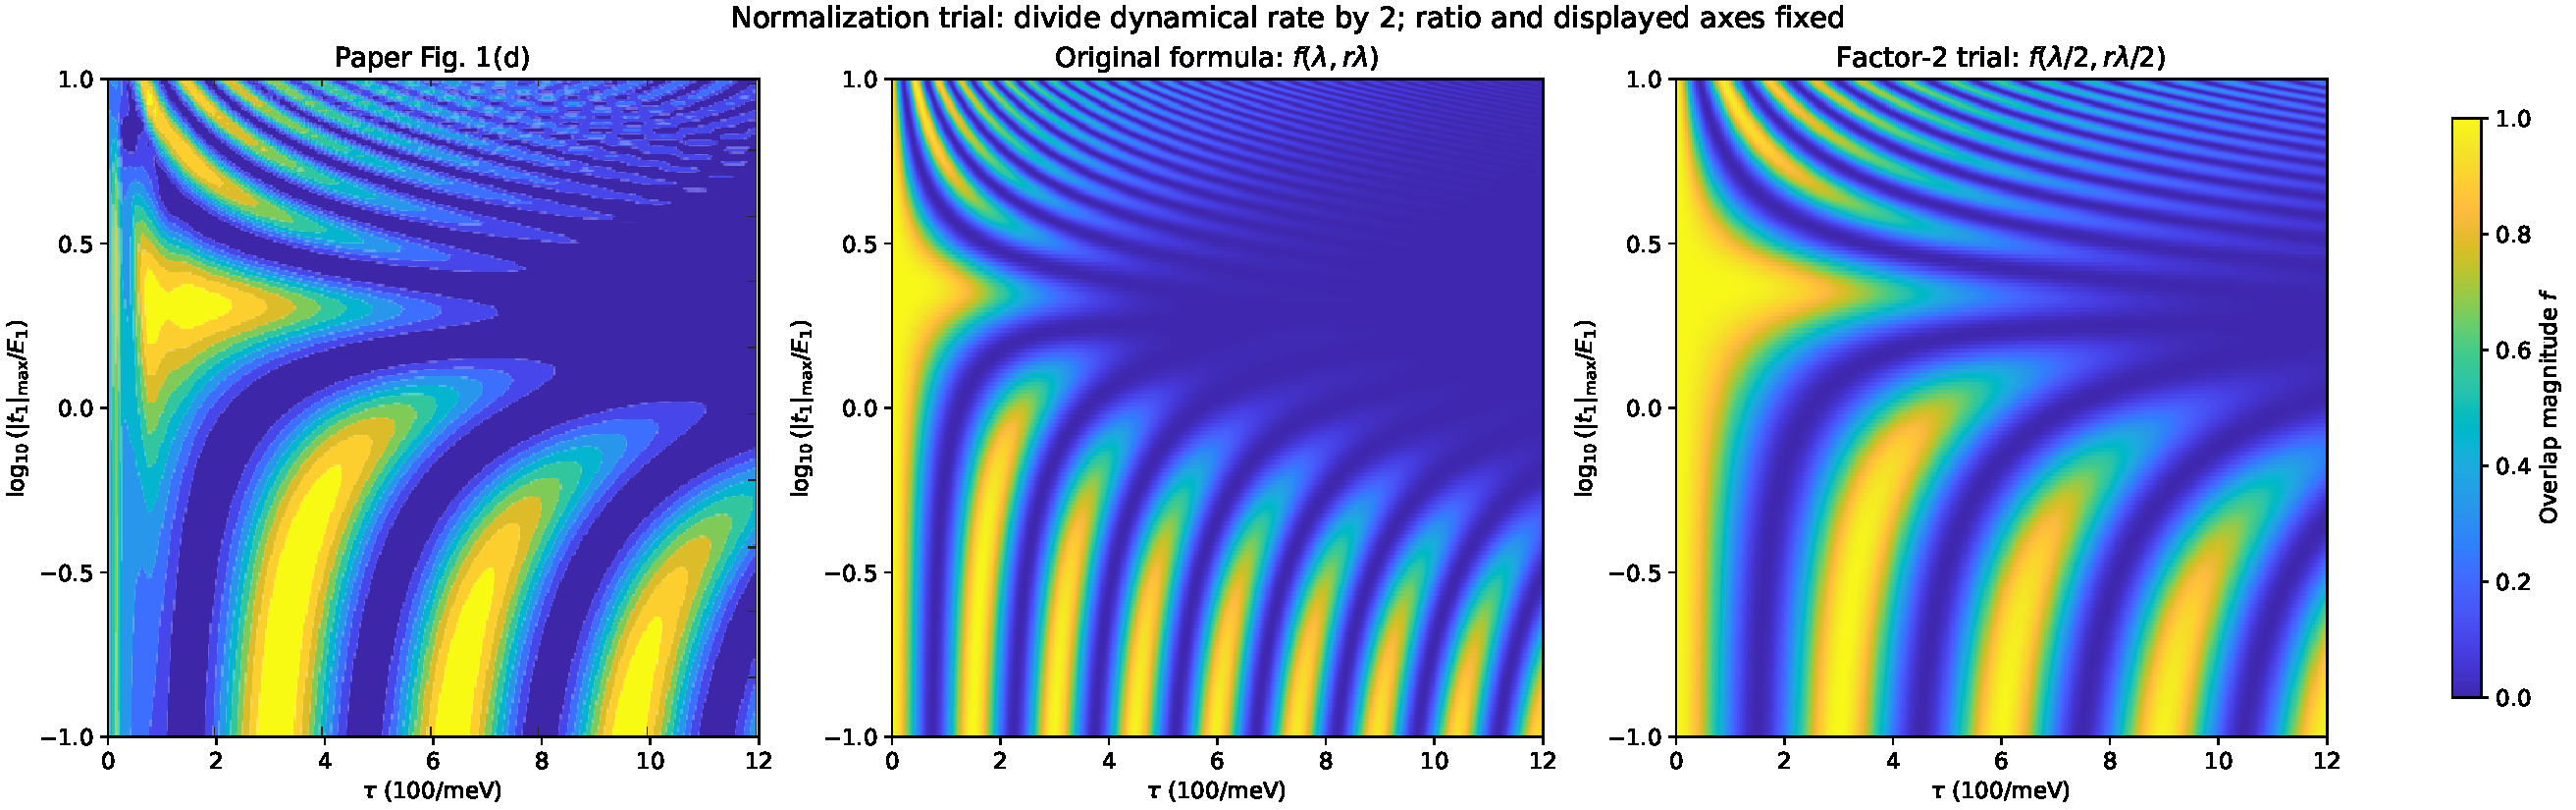
\includegraphics[width=\linewidth,height=4.2cm,keepaspectratio]{paper_vs_formula_factor2_trial.pdf}
  \end{center}
  \small
  试画采用 $f_{\rm trial}(\lambda,r)=\ff(\lambda/2,r\lambda/2)$，同时将两个累计角减半。
  \vspace{.18cm}
  \takeaway{保持比例 $r$ 和保真度幅值不变，仅观察动态速率变化后的峰数、峰宽；这项尝试尚未确定论文的归一化约定。}
\end{frame}

% 24 — brief §5: section cuts
\begin{frame}[t]{5. 图像与验证：固定比例截面对照}
  \begin{columns}[T,onlytextwidth]
    \begin{column}{.76\textwidth}
      \centering
      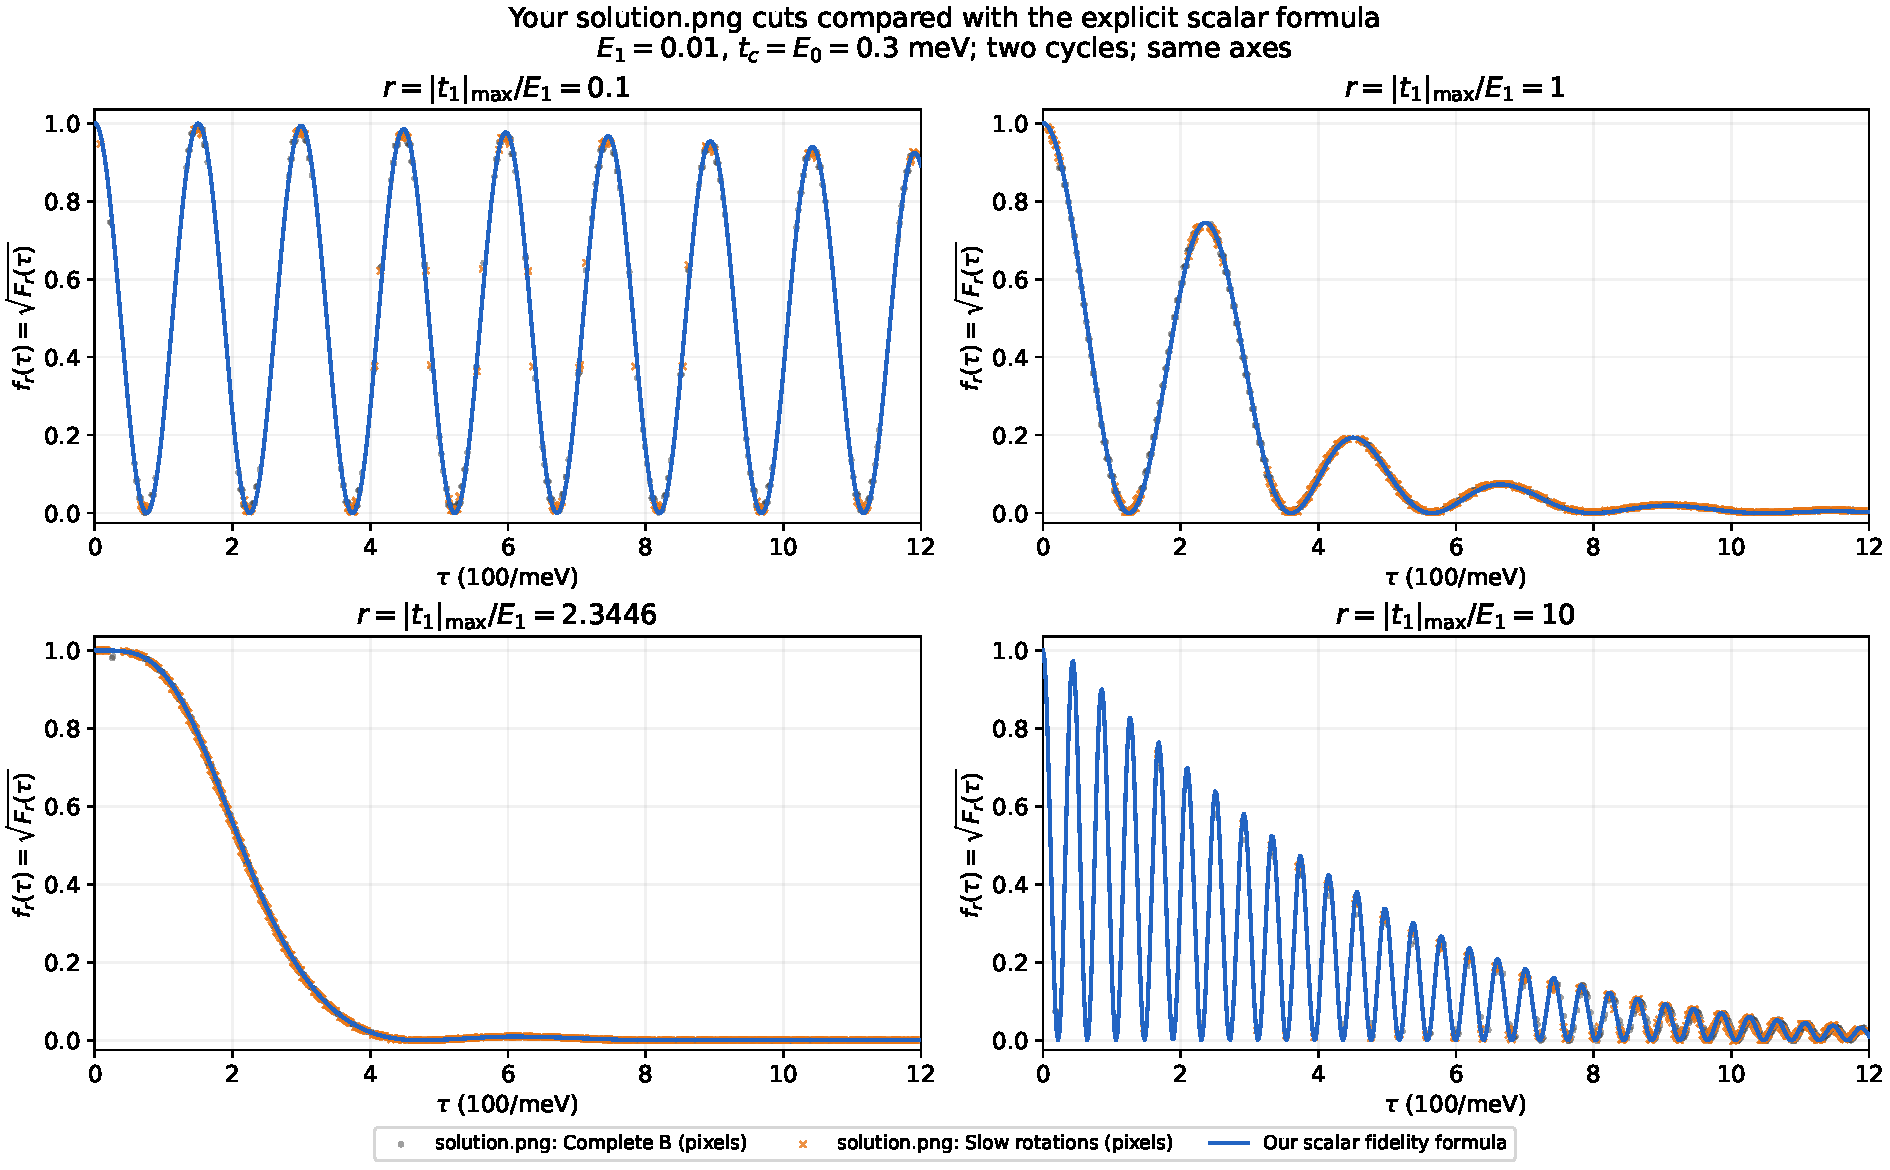
\includegraphics[width=\linewidth,height=5.3cm,keepaspectratio]{solution_vs_scalar_formula.pdf}
    \end{column}
    \begin{column}{.22\textwidth}
      \small
      截面就是同一函数：
      \[
        f_r(\lambda)=\ff(\lambda,r\lambda).
      \]
      没有重新拟合。\par\medskip
      蓝线为公式，散点来自已有 \texttt{solution.png}。\par\medskip
      源图像素含提取误差。
    \end{column}
  \end{columns}
\end{frame}

% 25 — brief §5: quantitative verification
\begin{frame}[t]{5. 图像与验证：完整模型数组的直接比较}
  $0.5\le\lambda\le12$，步长 $0.02$，比较已有完整模型数组与解析公式：
  \begin{center}
    \renewcommand{\arraystretch}{1.3}
    \begin{tabular}{cc}
      \toprule $r=\eta/E_1$ & 最大绝对差 $\max|f_{\rm full}-f_0|$\\\midrule
      $0.1$ & $0.00581$\\
      $1$ & $0.00547$\\
      $2.3446$ & $0.00185$\\
      $10$ & $0.04924$\\\bottomrule
    \end{tabular}
  \end{center}
  \small
  前三条截线的差值小于 $0.01$；$r=10$ 时 $\eta/C=1/3$，低能近似变弱。
  \vspace{.15cm}
  \begin{block}{另一种检查：公式求值本身}
    与独立低能微分方程比较，24 个测试点最大差约 $2.19\times10^{-9}$。
    这检验公式求值；上表检验低能近似，二者不能混同。
  \end{block}
  \source{有限网格验证不等于整张热图的统一精度保证。记录：verification.json、solution\_vs\_scalar\_formula.json。}
\end{frame}

\section{6. 近似条件与最终结论}

% 26 — brief §6
\begin{frame}[t]{6. 近似条件与最终结论}
  \small
  \setlength{\abovedisplayskip}{5pt}\setlength{\belowdisplayskip}{5pt}
  主要条件为
  \[
    \epsilon=\frac{\sqrt{E_1^2+\eta^2}}C\ll1,\qquad L=\frac{C\tau}{\hbar}\gg1.
  \]
  不要求 $\alpha,\nu\ll1$，但弱耦合高阶修正会随时间累积。在已证明的条件下，
  \[
    \boxed{f_{\rm full}=\ff(\alpha,\nu)+\Delta_{\rm phys},\qquad
      |\Delta_{\rm phys}|\le\min(1,\mathcal E_{\rm phys}).}
  \]
  \[
    \mathcal E_{\rm phys}
      =O\!\left(\epsilon^2+L\epsilon^3+\frac\epsilon L+\frac1{L^2}\right).
  \]
  \begin{itemize}\setlength{\itemsep}{.1cm}
    \item 物理上界较保守，大 $O$ 不等于已知数值系数。
    \item 绘图采用等价有序积分表示，截至第九阶的纯级数误差 $<1.42\times10^{-8}$。
    \item 该截断不是九阶累计角多项式，也不包含求积和物理投影误差。
  \end{itemize}
  \source{显式物理误差界及条件：技术文档第 17 节；绘图级数与截断界：第 7 节。}
\end{frame}

\end{document}
